\documentclass[conference,12pt]{IEEEtran}
\usepackage{pdflscape}
\usepackage{hyperref}
\usepackage{tabularx}
\usepackage{graphicx, subfigure, amsmath} 
\usepackage{pdfpages}
\usepackage[backend=biber,style=ieee]{biblatex}
%\usepackage[section]{placeins}
\addbibresource{References.bib}
\interdisplaylinepenalty=2500

% correct bad hyphenation here
\hyphenation{}


\begin{document}
%
% paper title
\title{Routing IPsec through NAT Gateways using Transport Mode}

\author{
\IEEEauthorblockN{Jeremy Wright}
\IEEEauthorblockA{Arizona State University\\jlwrigh1@asu.edu}
}
\maketitle
\begin{abstract}
Transport Mode IPsec provides a strongly secured means to connect two hosts
together. Either the Authentication Header (AH) and Encapsulated Security
Protocol can be used to implement varying levels of authentication and
confidentiality depending on the communication need. However, when communicating
on an IPv4 network, one must consider Network Address Translation (NAT) devices
translating local IP addresses to global IP addresses. Without extra
consideration this breaks end-to-end authentication. This paper discusses 
a UDP based solution to end-to-end confidential communication using IPsec transport mode.
\end{abstract}

\begin{IEEEkeywords}
    Transport Mode, Tunnel Mode, IPsec, NAT-T, UDP
\end{IEEEkeywords}

\section{Introduction}
IPsec is a layer 3 end-to-end security protocol for communicating over insecure
channels \autocite{rfc4301}, \autocite{_osi_2014}. As a layer 3 protocol
IPsec, offers a key advantage over security protocols at higher levels of abstractions
such as SSL/TLS. Application level security solutions require applications to be
designed with security in mind. IPsec secures the underlying transport providing
security services to any application. For some applications this is an
enormous advantage, especially for established applications which cannot be
extended to incorporate new security models. In this paper we will describe 
how to establish an end-to-end secure connection between to hosts as shown in Figure~\ref{fig:network}.

\begin{figure}
\centering
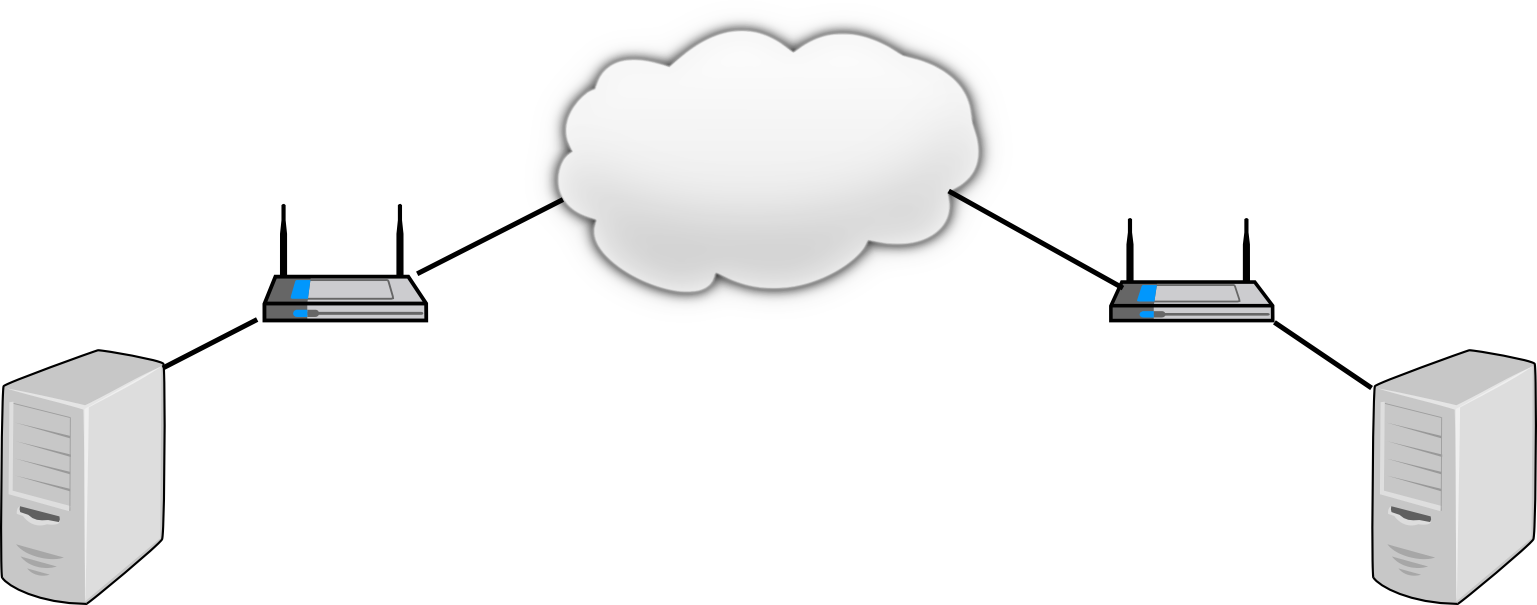
\includegraphics[width=0.4\textwidth]{network.png}
\caption{Example Network with two NAT gateways}
\label{fig:network}
\end{figure}

\section{IPsec}
IPsec defines two modes of operation transport mode, and tunnel mode. Primarily,
transport mode is used to establish host to host communication, while tunnel
mode is used to link two networks together, forming 1 larger network \autocite{cisco_ipsec}. IPsec 
defines 2 header types the Authentication Header, and Encapsulated Security
Protocol Header. Each header uses a HMAC based hash to preserve integrity of
various fields within the packet, however when using NAT the integrity is broken 
by NAT mutating source and destination fields \autocite{rfc3022}. Thus each header
authenticates different fields for its intended use case. 

As shown in Figure~\ref{fig:ah_example}, the Authentication Header provides no
confidentiality since its default mode does not support encryption.  Notice
that the application developer could encrypt their own data, but this defeats
the goal of IPsec providing a complete security model independent of the
application. 

Encapsulated Security Protocol Header (Figure~\ref{fig:esp_example}) however, does
provide confidentiality via an encrypted data payload. This packet
additionally provides mutable fields excluded from the HMAC calculation. However
this alone is insufficient to traverse two NAT gateways and simultaneously provide
authentication and confidentiality. IPv6
networks NAT is not necessary since all addresses are globally routable.
Within IPv4, NAT is required, but breaks end-to-end security since the
NAT cannot change the source or destination fields, and also preserve the integrity
of the packet. Tunnel mode provides a method for dealing with this, but does not
fit all use cases. 

\begin{figure}
\centering
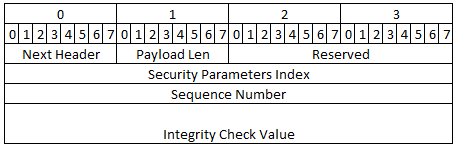
\includegraphics[width=0.4\textwidth]{AH.png}
\caption{IPsec: Authentication Header}
\label{fig:ah}
\end{figure}

\begin{figure}
\centering
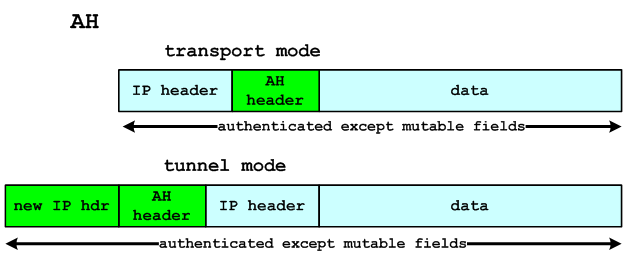
\includegraphics[width=0.4\textwidth]{AH_example.PNG}
\caption{Authentication Header \autocite{ipsec_example}}
\label{fig:ah_example}
\end{figure}

\begin{figure}
\centering
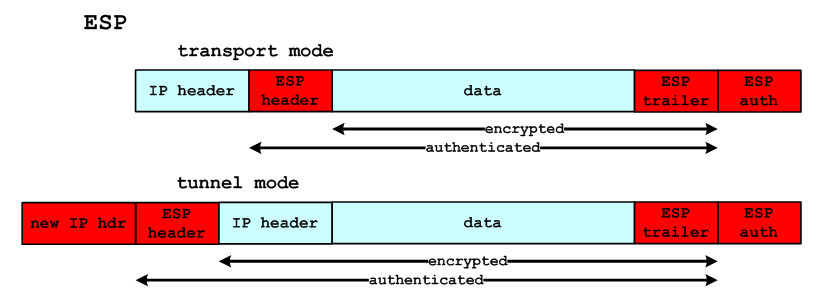
\includegraphics[width=0.4\textwidth]{ESP_example.PNG}
\caption{Encapsulated Security Protocol Header \autocite{ipsec_example}}
\label{fig:esp_example}
\end{figure}


Tunnel Mode uses the ESP header (Figure~\ref{fig:esp}) to wrap the desired IP
packet. The encapsulated IP package is encrypted, and the outer header defines
mutable, and immutable fields available for NAT \autocite{rfc4301}. While this
addresses the NAT issue, it ignores the fact that tunnel mode is primarily
intended for network to network connections.   

\begin{figure}
\centering
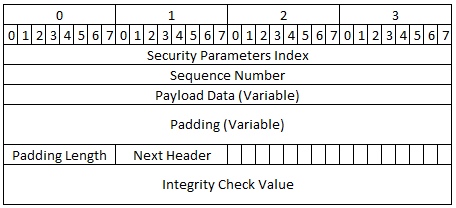
\includegraphics[width=0.4\textwidth]{ESP.png}
\caption{IPsec: Encapsulated Security Payload Header}
\label{fig:esp}
\end{figure}

\section{NAT-T Traversal}
RFC3947 provides a mechanism to use IPsec transport mode through a NAT gateway
\autocite{rfc3947}. However as noted in section 4 of this document, this doesn't
fully deal with the problem as it pushes requirements into the router software
to function properly. ``The best approach is simply to move the IKE traffic off port 500 
as soon as possible to avoid any IPsec-aware NAT special casing
\autocite{rfc3947}''.  This seems like a prime area for race
conditions, and contention issues as multiple services queue for port 500
access.  An alternative approach at the cost of
some additional overhead is to encapsulate the IPsec payload into a UDP packet.

\section{VPN with UDP Encapsulation}
UDP enables us to encapsulate the clients data in a standard packet type
routable by any standard router. Any NAT in the transport path can mutate the
fields of the outer packet without disrupting the integrity of the inner
encapsulated data. We can use the ESP header to provide confidentiality and
authentication as in Figure~\ref{fig:udp_encap}.  

\begin{figure}
\centering
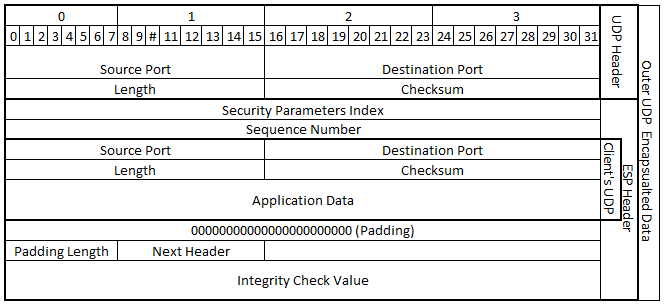
\includegraphics[width=0.4\textwidth]{UDP_encapsualted.PNG}
\caption{UDP Encapsulated Packet}
\label{fig:udp_encap}
\end{figure}

To establish our tunnel, we first must
establish where the encapsulation packing and unpacking occurs. For the
network defined in Figure~\ref{fig:network}, we have 3 options. 
\begin{enumerate}
\item Encapsulate packets in the switch.
\item Encapsulate packets in the user's operating system.
\item \label{item:sw} Encapsulate packets in a userspace software application running on the endpoint.
\end{enumerate}
For this use case we will assume the client is in a coffee shop or some similar
public network, hence the client cannot modify routing information in the switch.
Finally, the client wants to connect back to a desktop in a home office. For
this use case,
item~\ref{item:sw} is most fitting. The user can start the vpn software, enter
credentials and the software will establish the tunnel to the remote endpoint.

Since UDP will establish the tunnel we can use IPsec's transport mode. This
provides a clean division of responsibilities.  IPsec establishes security. UDP
establishes the tunnel.  IPsec protects all higher level protocols
(layers 4,5,6) without modification. Using an outer UDP packet, our software
application encapsulates VPN bound packets like
Figure~\ref{fig:udp_encap}.  The outer IPv4 packet is free to be manipulated
by any NAT within the pipeline. Whereas RFC 3947 requires a NAT discovery phase,
this encapsulated packet behaves as an ordinary IPv4 datagram. When the remote
host receives the outer IPv4 packet, it peels off the IPv4 and Outer UDP headers
to reveal a fully authenticated ESP datagram. The
application software then resumes routing the IPsec packet to its destination.
This defines our end-to-end secure channel.

\subsection{Routing our encapsulated header}
To route our header we will assume each router in Figure~\ref{fig:network}
provides NAT services.  The sender builds a datagram destined for the remote
host, say an
instant message professing the user's affinity for kittens
(Figure~\ref{fig:udp}). The application layer assembles the message as a UDP
packet and sends the datagram over its socket. Our VPN software receives the packets
since it's destined for the VPN secure connection.  

The VPN software assembles an ESP header and encrypts the UDP packet (Figure~\ref{fig:outer_ip}).  The IPsec
packet is routable at this point, but will not traverse a NAT.  To circumvent
the address translation, the VPN software builds a UDP packet to encapsulate the
ESP header (Figure~\ref{fig:outer_ip}).  The UDP packet is then encapsulated into the
IPv4 packet to route to the final network. The NAT is free to mutate it as required to get it to the
destination. Per RFC 6864 the identification field is not used
\autocite{rfc6864}. DSCP, and ECN
similarly are not used. The local router receives the packet and modifies the source address
 in the outer IPv4 header. Since the outer IPv4 packet is not included in the
 encapsulated ESP header's hash, integrity is not disrupted. This is what
 prevented us from using the ESP
header natively. 

On the receiving end, the remote NAT accepts the outer IPv4 packet and
translates the destination IP to an internal IP address via its internal
tables.  The remote host receives the datagram, and peels off the IPv4 and
UDP headers. It uses the UDP key as internal information.  The ESP header is
verified for integrity (which verifies the fields and data).  This integrity
check is a key benefit of ESP. Lastly, the data gram is
decrypted, and the resulting UDP packet is routed up to the application layer.


\begin{figure}
\centering
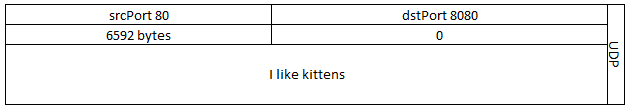
\includegraphics[width=0.4\textwidth]{udp_1.png}
\caption{UDP Packet the user wishes to send via VPN}
\label{fig:udp}
\end{figure}

\begin{figure}
\centering
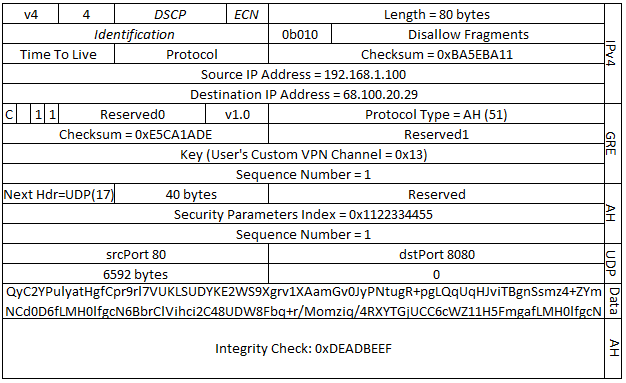
\includegraphics[width=0.4\textwidth]{ip4_4.png}
\caption{IPv4 Sending the UDP Packet}
\label{fig:outer_ip}
\end{figure}



\section{Conclusion}
Traditionally, when configuring IPsec, one would use Tunnel Mode to connect to
large networks together creating a larger virtual LAN. For remote users
connecting to a publicly accessible server, transport mode may be more useful.
However to create a secure connection between two end users in a peer-to-peer
fashion, one can look at defining
a new protocol based on UDP, to route their custom secure clients through
Network Address Translators. Since this approach operates at Layer 3, it has the
added benefit of providing secure communications to applications without
existing security. Their traffic is successfully encapsulated into the ESP, and
UDP headers to arrive at their destination, securely.



\printbibliography
\end{document}
